\documentclass[tikz,border=10pt]{standalone}
\usetikzlibrary{mindmap}

\begin{document}
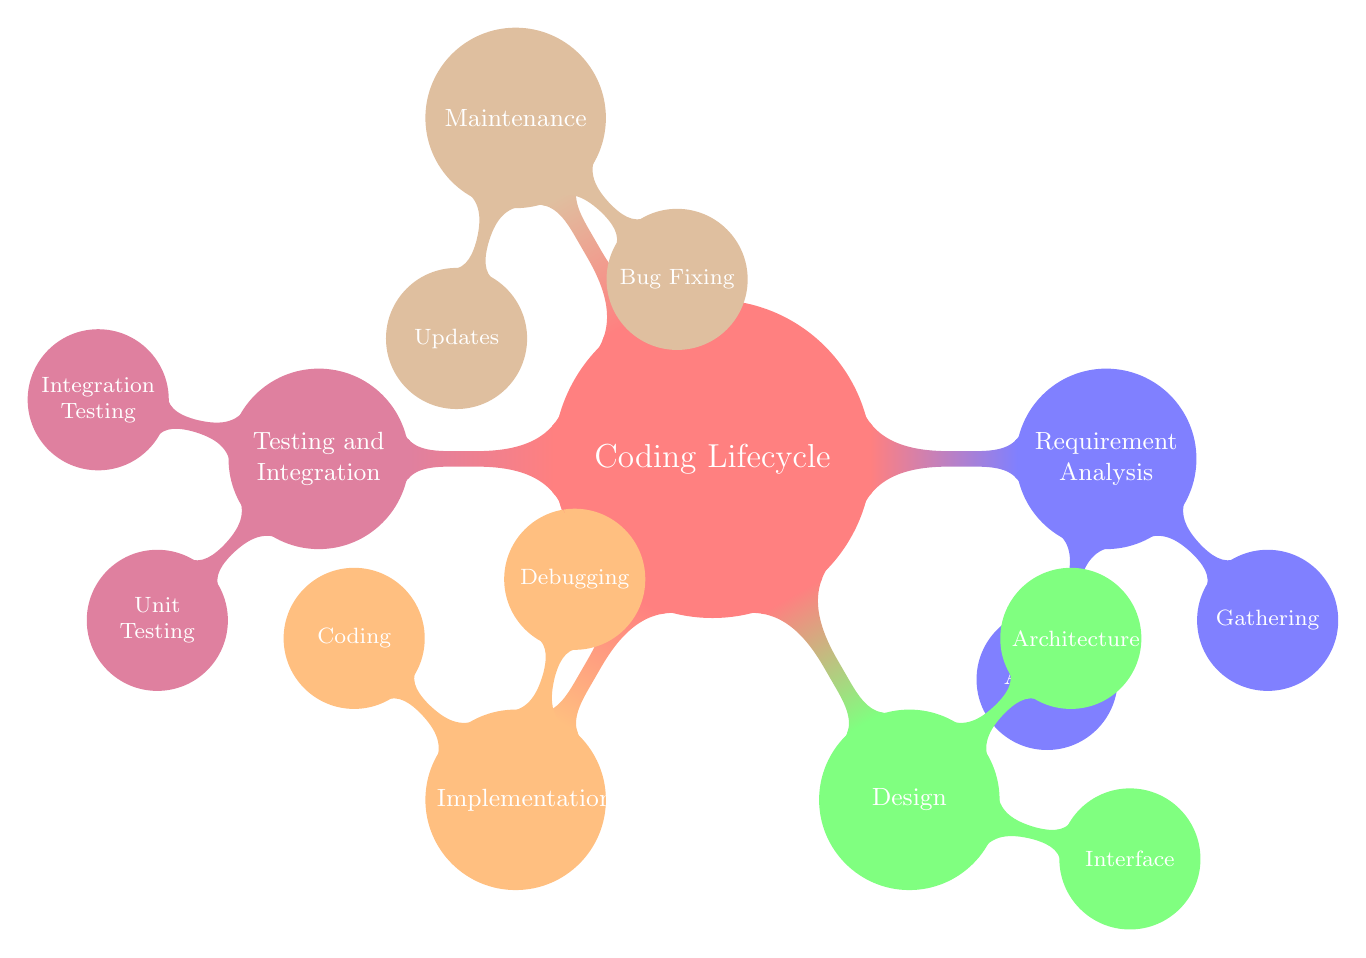
\begin{tikzpicture}
  \path[mindmap,concept color=red!50,text=white]
    node[concept] (root) {Coding Lifecycle}
    [clockwise from=0]
    child[concept color=blue!50] {
      node[concept] (ra) {Requirement Analysis}
      [clockwise from=-45]
      child {node[concept, concept color=blue!50] {Gathering}}
      child {node[concept, concept color=blue!50] {Analysis}}
    }
    child[concept color=green!50] {
      node[concept] (d) {Design}
      [clockwise from=45]
      child {node[concept, concept color=green!50] {Architecture}}
      child {node[concept, concept color=green!50] {Interface}}
    }
    child[concept color=orange!50] {
      node[concept] (i) {Implementation}
      [clockwise from=135]
      child {node[concept, concept color=orange!50] {Coding}}
      child {node[concept, concept color=orange!50] {Debugging}}
    }
    child[concept color=purple!50] {
      node[concept] (ti) {Testing and Integration}
      [clockwise from=-135]
      child {node[concept, concept color=purple!50] {Unit Testing}}
      child {node[concept, concept color=purple!50] {Integration Testing}}
    }
    child[concept color=brown!50] {
      node[concept] (m) {Maintenance}
      [clockwise from=-45]
      child {node[concept, concept color=brown!50] {Bug Fixing}}
      child {node[concept, concept color=brown!50] {Updates}}
    };
\end{tikzpicture}
\end{document}